\chapter{Materiais e métodos}\label{chap:materiais}

Este capítulo descreve os materiais, ferramentas, arquitetura, etapas de desenvolvimento, validação, cronograma, resultados esperados e limitações do trabalho. A metodologia foi definida a partir dos objetivos apresentados no \cref{chap:problema}, buscando demonstrar de forma verificável que o sistema proposto pode ser construído e avaliado em contexto acadêmico.

\section{Caracterização da pesquisa}

Este trabalho caracteriza-se como uma pesquisa aplicada, de natureza experimental e tecnológica, com desenvolvimento de um protótipo funcional. A abordagem combina estudo bibliográfico, implementação de sistema computacional e validação empírica por meio de cenários de teste em áreas agrícolas.

O método adotado não se limita à construção da aplicação. Ele define um conjunto de etapas necessárias para demonstrar que o objetivo foi atingido: definição da arquitetura, coleta de dados, implementação dos índices, desenvolvimento da interface, integração climática, testes funcionais, análise dos resultados e documentação das limitações.

\section{Ferramentas}

O sistema será desenvolvido com ferramentas gratuitas ou de amplo acesso acadêmico, conforme apresentado na \cref{tab:ferramentas}.

\begin{table}[htb!]
    \centering
    \caption{Ferramentas e recursos previstos para o desenvolvimento do protótipo.}
    \label{tab:ferramentas}
    \begin{tabular}{|l|p{9.5cm}|}
        \hline
        \textbf{Recurso} & \textbf{Função no projeto} \\ \hline
        Python & Linguagem principal de desenvolvimento. \\ \hline
        Streamlit & Interface web para interação com o usuário. \\ \hline
        Google Earth Engine & Consulta e processamento de imagens de satélite. \\ \hline
        Sentinel-2 Level-2A & Fonte principal de imagens multiespectrais. \\ \hline
        geemap & Integração entre Earth Engine e mapas interativos. \\ \hline
        Plotly & Geração de gráficos e séries temporais. \\ \hline
        pandas e numpy & Manipulação de dados e cálculos estatísticos. \\ \hline
        NASA POWER & Consulta de precipitação, temperatura e radiação solar. \\ \hline
        pytest & Testes automatizados do sistema. \\ \hline
    \end{tabular}
\end{table}

O protótipo deverá executar localmente em computador pessoal, com autenticação no Google Earth Engine por meio de variável de ambiente contendo o identificador do projeto. O processamento pesado das imagens será realizado no Earth Engine, reduzindo a necessidade de armazenamento local.

\section{Arquitetura proposta}

A arquitetura seguirá uma organização em três camadas: interface, processamento e dados externos. A \cref{fig:arquitetura} apresenta o fluxo geral de comunicação entre os componentes.

\begin{figure}[htb!]
    \centering
    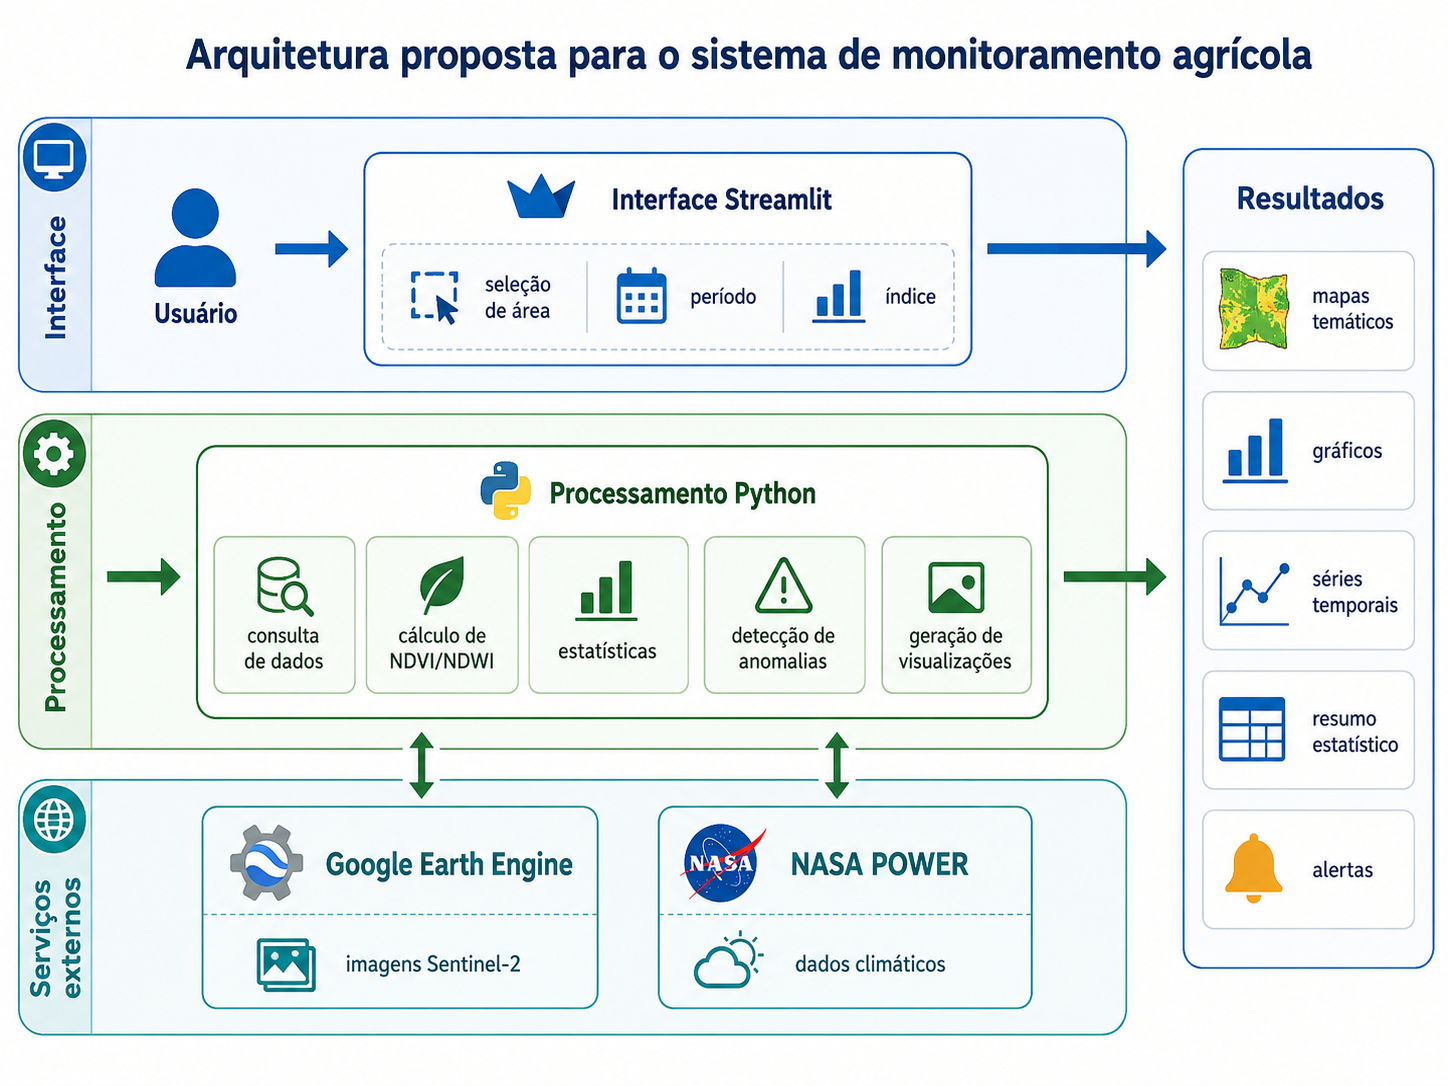
\includegraphics[width=0.92\textwidth]{fig/figura3.png}
    \caption{Arquitetura proposta para o sistema de monitoramento agrícola.}
    \label{fig:arquitetura}
    \vspace{0.2cm}
    \small Fonte: Elaborado pelo autor (2026).
\end{figure}

A camada de interface será responsável pela entrada de parâmetros e exibição dos resultados. A camada de processamento reunirá módulos Python responsáveis por autenticação, consulta de dados, cálculo de índices, séries temporais, anomalias e preparação dos gráficos. A camada de dados externos utilizará Google Earth Engine para imagens Sentinel-2 e NASA POWER para dados climáticos.

Essa arquitetura favorece modularidade, pois separa a interface da lógica de processamento. Também facilita testes automatizados, já que funções como cálculo de índices, geração de séries e detecção de anomalias podem ser validadas separadamente.

\section{Metodologia para o desenvolvimento}

O desenvolvimento será organizado em seis etapas principais, apresentadas na \cref{fig:metodologia}.

\begin{figure}[htb!]
    \centering
    \fbox{
    \begin{minipage}{0.92\textwidth}
        \centering
        Definição da arquitetura
        $\rightarrow$ Coleta de dados
        $\rightarrow$ Cálculo dos índices
        $\rightarrow$ Interface
        $\rightarrow$ Dados climáticos
        $\rightarrow$ Testes e validação
    \end{minipage}}
    \caption{Fluxo metodológico previsto para o desenvolvimento do protótipo.}
    \label{fig:metodologia}
\end{figure}

\subsection{Definição da arquitetura}

A primeira etapa consiste em definir os componentes do sistema, o fluxo de dados e as responsabilidades de cada módulo. Serão documentadas as entradas do usuário, as consultas externas, as estruturas de retorno e as visualizações esperadas.

\subsection{Coleta de dados de satélite}

As imagens serão obtidas a partir da coleção Sentinel-2 no Google Earth Engine. O sistema deverá receber a geometria da área de interesse, a data inicial e a data final. Em seguida, aplicará filtros de área, período e cobertura de nuvens.

Serão utilizadas principalmente as bandas B4, B8 e B11. A banda B4 corresponde ao vermelho e será usada no NDVI. A banda B8 corresponde ao infravermelho próximo e será usada no NDVI e no NDWI. A banda B11 corresponde ao infravermelho de ondas curtas e será usada no NDWI.

Os metadados relevantes, como data de aquisição, percentual de nuvens e identificador da imagem, deverão ser preservados para rastreabilidade.

\subsection{Cálculo de índices espectrais}

Para cada imagem válida, o sistema calculará NDVI e NDWI por meio de operações de diferença normalizada. Os resultados serão mantidos como bandas derivadas e utilizados em duas frentes: geração de mapa temático para visualização espacial e cálculo de estatísticas médias na área de interesse para composição de série temporal.

As estatísticas previstas incluem média, mediana, mínimo, máximo e desvio padrão, quando aplicável.

\subsection{Desenvolvimento da interface}

A interface será implementada em Streamlit. Ela deverá permitir selecionar ou desenhar a área de interesse, definir data inicial e data final, escolher o índice a ser analisado, executar a análise, visualizar mapa temático, visualizar gráfico de série temporal, consultar resumo estatístico, visualizar alerta de anomalia e visualizar dados climáticos associados ao período.

Como o objetivo é um MVP acadêmico, não serão incluídos cadastro de usuários, banco de dados complexo, controle de permissões ou aplicação móvel.

\subsection{Integração de dados climáticos}

O sistema consultará a NASA POWER usando a coordenada central da área de interesse e o mesmo intervalo temporal escolhido para as imagens. As variáveis inicialmente previstas são precipitação diária, temperatura média diária e radiação solar de superfície.

Os dados serão convertidos para tabela e exibidos em gráficos. A interpretação será feita de forma comparativa, observando se oscilações nos índices coincidem com eventos climáticos relevantes.

\subsection{Detecção de anomalias}

A detecção de anomalias será baseada em série temporal. O critério inicial utilizará média móvel e desvio padrão. Um ponto poderá ser marcado como anômalo quando apresentar queda inferior a um limiar definido, como um desvio padrão abaixo da média da janela anterior.

Esse método foi escolhido por ser simples, interpretável e adequado ao escopo de um protótipo. Sua limitação é que ele não identifica a causa da anomalia e pode ser sensível ao tamanho da janela, à quantidade de imagens disponíveis e à presença de ruídos.

\section{Validação}

A validação será realizada em três níveis. O primeiro nível envolve testes automatizados para verificar funções de configuração, autenticação, cálculo de índices, estrutura de retorno e tratamento de erros. O segundo envolve testes funcionais, nos quais o fluxo completo será executado desde a seleção da área até a exibição dos resultados. O terceiro envolve validação interpretativa, com comparação de séries e mapas com faixas esperadas de NDVI e NDWI, observando o comportamento de áreas de soja, milho e pastagem.

O sistema será considerado funcional se conseguir retornar mapas, séries temporais, dados climáticos e alertas sem falhas impeditivas para entradas válidas. Os cenários agrícolas previstos para validação são apresentados na \cref{tab:cenarios}.

\begin{table}[htb!]
    \centering
    \caption{Cenários agrícolas previstos para validação do protótipo.}
    \label{tab:cenarios}
    \begin{tabular}{|l|p{10.5cm}|}
        \hline
        \textbf{Cenário} & \textbf{Característica esperada} \\ \hline
        Soja & Aumento de NDVI durante o desenvolvimento vegetativo e redução no final do ciclo. \\ \hline
        Milho & Crescimento gradual do NDVI até o pico vegetativo, com posterior queda. \\ \hline
        Pastagem & Valores relativamente estáveis, com variações associadas a clima e manejo. \\ \hline
    \end{tabular}
\end{table}

As áreas deverão ser definidas durante a execução do projeto. Caso não existam dados de campo disponíveis, a validação ficará limitada à coerência dos índices, comparação com literatura e análise visual das séries temporais.

\section{Cronograma}\label{sec:cronograma}

O cronograma considera a execução do trabalho entre julho e dezembro de 2026. Cada mês é dividido em quatro semanas, conforme apresentado na \cref{tab:cronograma}.

\begin{table}[htb!]
\centering
\small
\caption{Cronograma de atividades da proposta de Trabalho de Conclusão.}
\label{tab:cronograma}
\begin{tabular}{|p{5.3cm}|c|c|c|c|c|c|}
\hline
\textbf{Atividade} & \textbf{Jul} & \textbf{Ago} & \textbf{Set} & \textbf{Out} & \textbf{Nov} & \textbf{Dez} \\ \hline
Definição da arquitetura & S1--S4 & & & & & \\ \hline
Coleta de dados Sentinel-2 & S3--S4 & S1--S4 & & & & \\ \hline
Implementação de NDVI e NDWI & & S3--S4 & S1--S4 & & & \\ \hline
Desenvolvimento da interface & & & S3--S4 & S1--S4 & S1--S2 & \\ \hline
Integração de dados climáticos & & & & S3--S4 & S1--S4 & \\ \hline
Testes e validação & & & & & S3--S4 & S1--S4 \\ \hline
Análise e discussão dos resultados & & & & S4 & S1--S4 & S1 \\ \hline
Elaboração do texto final & & & & S3--S4 & S1--S4 & S1--S3 \\ \hline
Preparação para defesa & & & & & & S1--S4 \\ \hline
Banca de defesa & & & & & & S4 \\ \hline
\end{tabular}
\end{table}

A definição da arquitetura compreenderá a documentação dos componentes, fluxo de dados, tecnologias e interfaces entre módulos. A coleta de dados envolverá a configuração do Earth Engine, seleção de áreas, consulta às imagens Sentinel-2 e filtragem por data e nuvem.

A implementação dos índices abrangerá a criação das funções de NDVI e NDWI, geração de mapas temáticos e cálculo de estatísticas para séries temporais. O desenvolvimento da interface incluirá controles de entrada, mapa interativo, gráficos e painel de resumo.

A integração climática envolverá a consulta à NASA POWER e a associação dos dados de clima ao período analisado. Os testes e validação verificarão o funcionamento do fluxo completo, a coerência dos valores calculados e a detecção de anomalias. A análise e discussão dos resultados organizará os achados, limitações e interpretações. A elaboração do texto final ocorrerá em paralelo às últimas etapas, com revisão contínua e preparação para a defesa.

\section{Resultados esperados}

Espera-se obter um protótipo funcional capaz de consultar imagens Sentinel-2 para uma área e período definidos, calcular NDVI e NDWI, gerar mapas temáticos dos índices, produzir séries temporais, consultar dados climáticos, indicar possíveis anomalias e apresentar resultados em interface web simples.

Também se espera produzir documentação técnica e acadêmica suficiente para explicar as decisões de arquitetura, as limitações do protótipo e os caminhos de evolução. O resultado esperado não é um produto comercial completo, mas uma prova de conceito funcional e reproduzível para o contexto acadêmico.

\section{Limitações}

O trabalho possui limitações importantes. A resolução espacial do Sentinel-2 permite análise de talhões, mas não de plantas individuais. A presença de nuvens, sombras e falhas de aquisição pode reduzir a quantidade de imagens úteis. Os índices espectrais indicam padrões de vegetação, mas não identificam diretamente pragas, doenças, deficiência nutricional ou causa exata de estresse.

Além disso, a validação poderá ser limitada pela ausência de dados de campo. Nesse caso, a análise será baseada em coerência espectral, comparação com faixas esperadas e relação temporal com dados climáticos. O sistema também não pretende ser produto comercial completo, pois não incluirá autenticação de usuários, banco de dados robusto, aplicativo móvel, integração com sensores de campo ou diagnóstico agronômico automatizado.

\section{Trabalhos futuros}

Como evolução, o sistema poderá incluir suporte a novos índices, como NDMI, SAVI e EVI; integração com dados de drones ou sensores IoT; armazenamento histórico das análises; cadastro de usuários e propriedades; comparação entre talhões; modelos de aprendizado de máquina para classificação de anomalias; alertas automáticos; validação com dados de campo; e integração com bases meteorológicas locais, como INMET.
